\section{Metodologia}

\begin{frame}
  \frametitle{Amostragem}
 \begin{center}
  Pontos de amostragem em Nima:
 \end{center}
  \begin{figure}[H]
    \centering
    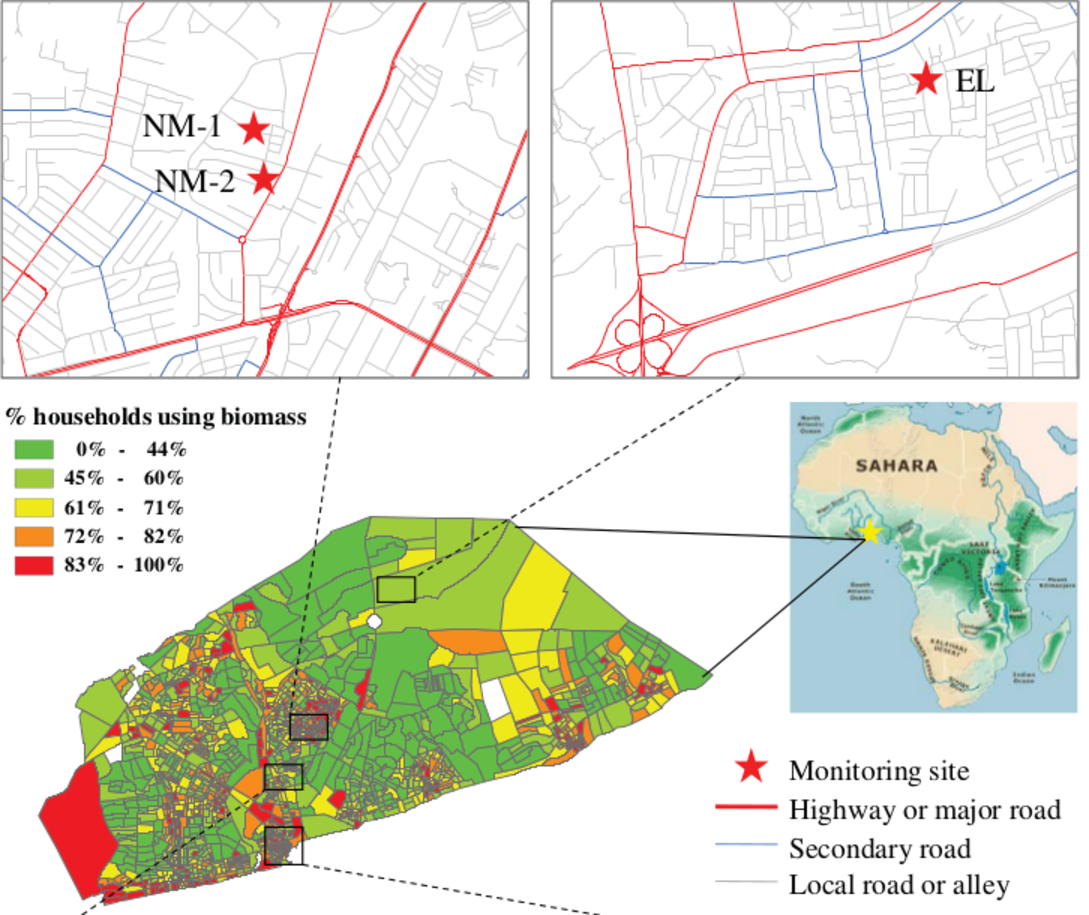
\includegraphics[scale=0.35]{../../inputs/images/zheng/nima_mapa.pdf}
  \end{figure}
\end{frame}

\begin{frame}
  \frametitle{Amostragem}
  \begin{figure}[H]
  \centering	
  \includegraphics[width=0.7\textwidth]{../../outputs/accra_sources.pdf}
  \caption{Levantamento de algumas fontes poluidora de Acra.
           \label{fg:acrasources}}
 \end{figure}
\end{frame}

\begin{frame}
  \frametitle{Dados da amostragem}
  \begin{itemize}
    \item Entre 11 de novembro de 2006 e 15 de agosto de 2008;
    \item 48 horas de amostragem;
    \item 2898 amostras coletadas de $MP_{10}$ e $MP_{2,5}$;
    \item Onze sítios localizados em quatro bairros diferentes;
    \item 879 amostras referem-se ao bairro de Nima
  \end{itemize}
\end{frame}

\begin{frame}
  \frametitle{Censo populacional}
\begin{center}
  Fonte de energia na preparação alimentos em Gana:
\end{center}
  \begin{table}[H]
  	\centering
  	\begin{tabular}{llrlr}
  \hline
  \multicolumn{1}{c}{Tipo da} & \multicolumn{2}{c}{Gana (todo país)} & \multicolumn{2}{c}{Acra}                                                           \\
  \multicolumn{1}{c}{fonte de energia} & 2000 & 2010 &  2000 & 2010  \\ 
 \hline & \multicolumn{4}{c}{\% de uso} \\ 
  \hline
  não cozinha           & 3,5 & 5,60 & 4,8 & 6,90 \\ 
\textcolor{red}{biomassa}              & \textcolor{red}{55,8} & \textcolor{red}{40,20} & \textcolor{red}{8,8} & \textcolor{red}{3,50} \\ 
\textcolor{blue}{gás}& \textcolor{blue}{6,2} & \textcolor{blue}{18,20} & \textcolor{blue}{21,8} & \textcolor{blue}{41,40} \\ 
  eletricidade          & 1,1 & 0,50 & 2,2 & 0,90 \\ 
  querosene             & 2 & 0,50 & 4,3 & 1,10 \\ 
 \textcolor{red}{carvão} & \textcolor{red}{30} & \textcolor{red}{33,70} & \textcolor{red}{57,3} & \textcolor{red}{45,40} \\ 
  resíduo de plantação  & * & 0,80 & * & 0,10 \\ 
  pó de serra           & * & 0,10 & * & 0,30 \\ 
  esterco               & * & 0,00 & * & 0,10 \\ 
  outros                & 1,1 & 0,10 & 0,8 & 0,30 \\ 
  \hline
\end{tabular}


  \end{table}
\end{frame}

\begin{frame}
  \frametitle{}
  Ilustração clássica do fenômeno de fluorescência de raios X no átomo.\\
  Transições de elétrons entre os subníveis das camadas K, L e M. 
  \begin{figure}[H]
    \centering
    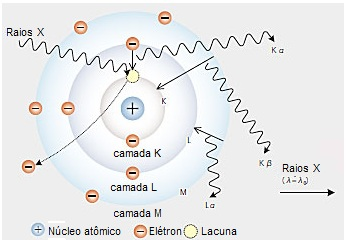
\includegraphics[width=0.4\textwidth]{../../inputs/images/shimadzu_atomo.jpg}
    \hspace{1cm}
    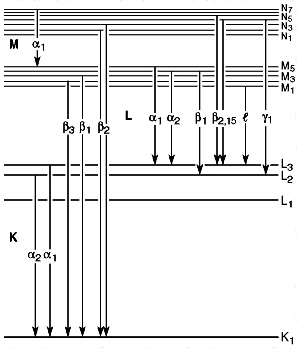
\includegraphics[width=0.4\textwidth]{../../inputs/images/Siegbahn.jpg}
  \end{figure}
\end{frame}

\begin{frame}
  \frametitle{Fluorescência de Raios X - \textit{ED-XRF}}
  Modelamento matemático usado na \textit{ED-XRF}:
  \begin{equation*}
    \label{eq:contagem}
    N(Z) = R(Z) \cdot I \cdot \Delta t  \cdot \frac{m(Z)}{A}
  \end{equation*}
  Onde,  
  \begin{itemize}
    \item N(Z) = Contagem de fótons na amostra para o elemento químico Z;
    \item I = Corrente (ampère) na amostra;
    \item $\Delta t$ = Tempo vivo (segundos) que a amostra foi irradiada;
    \item m(Z) = Massa na amostra para o elemento químico Z;
    \item A = Área amostrada do filtro.
  \end{itemize}
\end{frame}

\begin{frame}
  \frametitle{Calibração: Ajuste do Fator de Resposta}
  Constante de proporcionalidade: Fator de Resposta:
\begin{equation*}
  \label{eq:fator_de_resposta}
  R(Z) = \frac{N(Z)}{d(Z) \cdot I \cdot \Delta t}
\end{equation*}

\begin{equation*}
  \label{eq:erro_fator_de_resposta}
  \sigma_{R(Z)}^2 = {R(Z)}^2 \cdot \left[ \left(\frac{\sigma_{N(Z)}}{N(Z)}\right)^2 + 
                                      \left(\frac{\sigma_{d(Z)}}{d(Z)}\right)^2 
                                   \right]
\end{equation*}
\end{frame}

\begin{frame}
  \frametitle{Calibração: Ajuste do Fator de Resposta}
  Constante de proporcionalidade: Fator de Resposta:
\begin{equation*}
  \label{eq:xrfedmassa}
  m(Z) = \frac{N(Z) \cdot A}{ R(Z) \cdot I \cdot \Delta t}
\end{equation*}

\begin{equation*}
  \label{eq:erro_massa}
  \sigma_{m(Z)}^2 = {m(Z)}^2 \left[ \left(\frac{\sigma_{N(Z)}}{N(Z)}\right)^2 + 
                                  \left(\frac{\sigma_A}{A}\right)^2 + 
                                  \left(\frac{\sigma_{R(Z)}}{R(Z)}\right)^2 
                             \right]
\end{equation*}
\end{frame}

\begin{frame}
  \frametitle{Mínimos Quadrados Matricial}
\begin{equation*}
  \label{eq:polinomio}
  \begin{split}
    y_1 = a + b x_1 + c{x_1}^2 + d{x_1}^3 + ...\\
    y_2 = a + b x_2 + c{x_2}^2 + d{x_2}^3 + ... \\
    ...
  \end{split}
\end{equation*}

\begin{equation*}
  \label{eq:polinomioMatriz}
  [Y] = [A] \cdot [X]
\end{equation*}

Os coeficientes ajustados [Ã] são dados por:
\begin{equation*}
  [\tilde{A}] = [V_{\tilde{A}}] \cdot ([X]^T \cdot {[V_Y]}^{-1} \cdot [Y])
\end{equation*}

Sendo $[V_{\tilde{A}}]$ a matriz de covariância dos coeficientes, dada por:
\begin{equation*}
  [V_{\tilde{A}}] = ([X]^T [V_Y]^{-1} [X])^{-1}
\end{equation*}
\end{frame}

\begin{frame}
  \frametitle{Mínimos Quadrados Matricial}
A partir dos coeficientes ajustados [Ã] na equação \ref{eq:coeficientesajustados},
pode-se calcular os $[\tilde{Y}]$ ajustados,

\begin{equation*}
  \label{eq:polinomioajustado}
  [\tilde{Y}] = [\tilde{A}]\cdot[X]
\end{equation*}

A diagonal da matriz de covariância de $[\tilde{Y}]$, $[V_{\tilde{Y}}]$, 
representa a incerteza dos valores ajustados:

\begin{equation*}
  \label{eq:matrizcovarianciaY}
  [V_{\tilde{Y}}] = [X] \cdot [V_{\tilde{A}}]^{-1} \cdot [X]^{-1}
\end{equation*}

\end{frame}

\begin{frame}
  \frametitle{Modelo receptor}
  \textbf{Modelo Receptor} é uma abordagem matemática para quantificar o efeito das fontes 
  nas amostras. Determinar as fontes a partir do receptor. \\
  \textbf{Análise Multivariada} reduz as dimensões (variáveis) de um conjunto de dados 
  em um conjunto de dados analítico complexo que poderão ser interpretados como 
  tipo de fontes.
\end{frame}

\begin{frame}
  \frametitle{Conservação de massa}
  Fundamentação do modelo receptor: Conservação de massa. \\
  Todos modelos resolvem a mesma equação: 
  \begin{equation*}
    x_{ij} = \sum_{p=1}^{P} g_{ip}f_{pj} + \epsilon_{ij}
  \end{equation*} 
 
  \begin{itemize}
    \item $x_{ij}$ = concentração na amostra i da espécie j;
    \item $f_{pj}$ = fração da espécie j emitida na fonte p 
                    (perfil da fonte, assinatura da fonte ou \textit{Factor Loadings}); 
    \item $g_{ip}$ = contribuição da fonte p para amostra i (\textit{Factor Score});
    \item $\epsilon$ = Resíduo, depende do modelo empregado.
  \end{itemize}
\end{frame}

\begin{frame}
  \frametitle{Análise de Fatores}
  \begin{equation*}
    z_{j} = l_{j1}F_1 + l_{j2}F_2 + l_{j3}F_3 + ... + \epsilon_{ij}
  \end{equation*}
  \begin{itemize}
    \item $z_{j}$ = concentração da espécie j normalizada;
    \item Cálculo da matriz de correlação/covariância
    \item Extração de autovalores e autovetores (ortogonais). 
    \item Transformada Linear nos novos eixos
    \item $l_{jk}$ = contribuição da Fonte $F_k$
  \end{itemize}

\end{frame}


\begin{frame}
  \frametitle{Positive Matrix Factorizarion}

  Função objeto - Q -  é uma função que precisa ser minimizada. 
 
  \begin{equation*}
    Q = \sum_{i=1}^n \sum_{j=1}^m  \left[ \frac{ x_{ij} - \sum_{p=1}^{P} g_{ip}f_{pj}} {u_{ij}} \right] ^2
  \end{equation*}

  Diferente da Análise de Fatores, no PMF, a incerteza ($u_{ij}$) entra na conta.
\end{frame}

